% AUTO-GENERATED by code/figlib.py helpers -- do not edit
\nTenFit{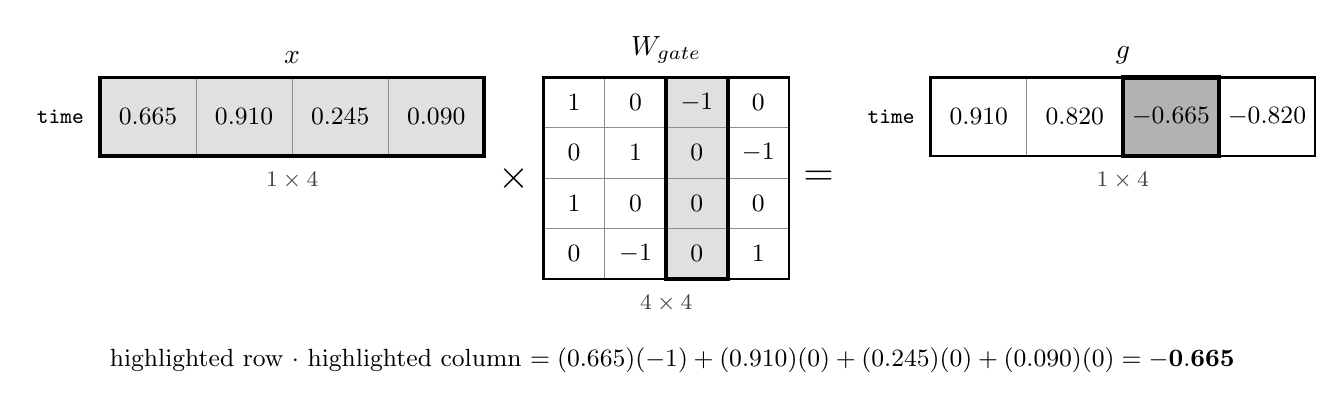
\begin{tikzpicture}
\draw[black!45, fill=black!12] (0.000,0.000) rectangle (1.220,-1.000);
\node[font=\small, text=black] at (0.610,-0.500) {$0.665$};
\draw[black!45, fill=black!12] (1.220,0.000) rectangle (2.440,-1.000);
\node[font=\small, text=black] at (1.830,-0.500) {$0.910$};
\draw[black!45, fill=black!12] (2.440,0.000) rectangle (3.660,-1.000);
\node[font=\small, text=black] at (3.050,-0.500) {$0.245$};
\draw[black!45, fill=black!12] (3.660,0.000) rectangle (4.880,-1.000);
\node[font=\small, text=black] at (4.270,-0.500) {$0.090$};
\draw[line width=1.4pt] (0.000,0.000) rectangle (4.880,-1.000);
\draw[line width=0.9pt] (0.000,0.000) rectangle (4.880,-1.000);
\node[anchor=east, font=\footnotesize\ttfamily] at (-0.080,-0.500) {time};
\node[anchor=south, font=\normalsize] at (2.440,0.050) {$\bm{x}$};
\node[anchor=north, font=\footnotesize, text=black!75] at (2.440,-1.080) {$1\times4$};
\draw[black!45, fill=white] (5.630,0.000) rectangle (6.410,-0.640);
\node[font=\small, text=black] at (6.020,-0.320) {$1$};
\draw[black!45, fill=white] (6.410,0.000) rectangle (7.190,-0.640);
\node[font=\small, text=black] at (6.800,-0.320) {$0$};
\draw[black!45, fill=black!12] (7.190,0.000) rectangle (7.970,-0.640);
\node[font=\small, text=black] at (7.580,-0.320) {$-1$};
\draw[black!45, fill=white] (7.970,0.000) rectangle (8.750,-0.640);
\node[font=\small, text=black] at (8.360,-0.320) {$0$};
\draw[black!45, fill=white] (5.630,-0.640) rectangle (6.410,-1.279);
\node[font=\small, text=black] at (6.020,-0.959) {$0$};
\draw[black!45, fill=white] (6.410,-0.640) rectangle (7.190,-1.279);
\node[font=\small, text=black] at (6.800,-0.959) {$1$};
\draw[black!45, fill=black!12] (7.190,-0.640) rectangle (7.970,-1.279);
\node[font=\small, text=black] at (7.580,-0.959) {$0$};
\draw[black!45, fill=white] (7.970,-0.640) rectangle (8.750,-1.279);
\node[font=\small, text=black] at (8.360,-0.959) {$-1$};
\draw[black!45, fill=white] (5.630,-1.279) rectangle (6.410,-1.919);
\node[font=\small, text=black] at (6.020,-1.599) {$1$};
\draw[black!45, fill=white] (6.410,-1.279) rectangle (7.190,-1.919);
\node[font=\small, text=black] at (6.800,-1.599) {$0$};
\draw[black!45, fill=black!12] (7.190,-1.279) rectangle (7.970,-1.919);
\node[font=\small, text=black] at (7.580,-1.599) {$0$};
\draw[black!45, fill=white] (7.970,-1.279) rectangle (8.750,-1.919);
\node[font=\small, text=black] at (8.360,-1.599) {$0$};
\draw[black!45, fill=white] (5.630,-1.919) rectangle (6.410,-2.558);
\node[font=\small, text=black] at (6.020,-2.239) {$0$};
\draw[black!45, fill=white] (6.410,-1.919) rectangle (7.190,-2.558);
\node[font=\small, text=black] at (6.800,-2.239) {$-1$};
\draw[black!45, fill=black!12] (7.190,-1.919) rectangle (7.970,-2.558);
\node[font=\small, text=black] at (7.580,-2.239) {$0$};
\draw[black!45, fill=white] (7.970,-1.919) rectangle (8.750,-2.558);
\node[font=\small, text=black] at (8.360,-2.239) {$1$};
\draw[line width=1.4pt] (7.190,0.000) rectangle (7.970,-2.558);
\draw[line width=0.9pt] (5.630,0.000) rectangle (8.750,-2.558);
\node[anchor=south, font=\normalsize] at (7.190,0.050) {$W_{\text{gate}}$};
\node[anchor=north, font=\footnotesize, text=black!75] at (7.190,-2.638) {$4\times4$};
\draw[black!45, fill=white] (10.550,0.000) rectangle (11.770,-1.000);
\node[font=\small, text=black] at (11.160,-0.500) {$0.910$};
\draw[black!45, fill=white] (11.770,0.000) rectangle (12.990,-1.000);
\node[font=\small, text=black] at (12.380,-0.500) {$0.820$};
\draw[black!45, fill=black!30] (12.990,0.000) rectangle (14.210,-1.000);
\node[font=\small, text=black] at (13.600,-0.500) {$-0.665$};
\draw[black!45, fill=white] (14.210,0.000) rectangle (15.430,-1.000);
\node[font=\small, text=black] at (14.820,-0.500) {$-0.820$};
\draw[line width=1.6pt] (12.990,0.000) rectangle (14.210,-1.000);
\draw[line width=0.9pt] (10.550,0.000) rectangle (15.430,-1.000);
\node[anchor=east, font=\footnotesize\ttfamily] at (10.470,-0.500) {time};
\node[anchor=south, font=\normalsize] at (12.990,0.050) {$\bm{g}$};
\node[anchor=north, font=\footnotesize, text=black!75] at (12.990,-1.080) {$1\times4$};
\node[font=\Large] at (5.255,-1.279) {$\times$};
\node[font=\Large] at (9.125,-1.279) {$=$};
\node[anchor=north west, font=\small] at (0,-3.308) {highlighted row $\cdot$ highlighted column $= (0.665)(-1) + (0.910)(0) + (0.245)(0) + (0.090)(0) = \mathbf{-0.665}$};
\end{tikzpicture}}
\\[10pt]
\nTenFit{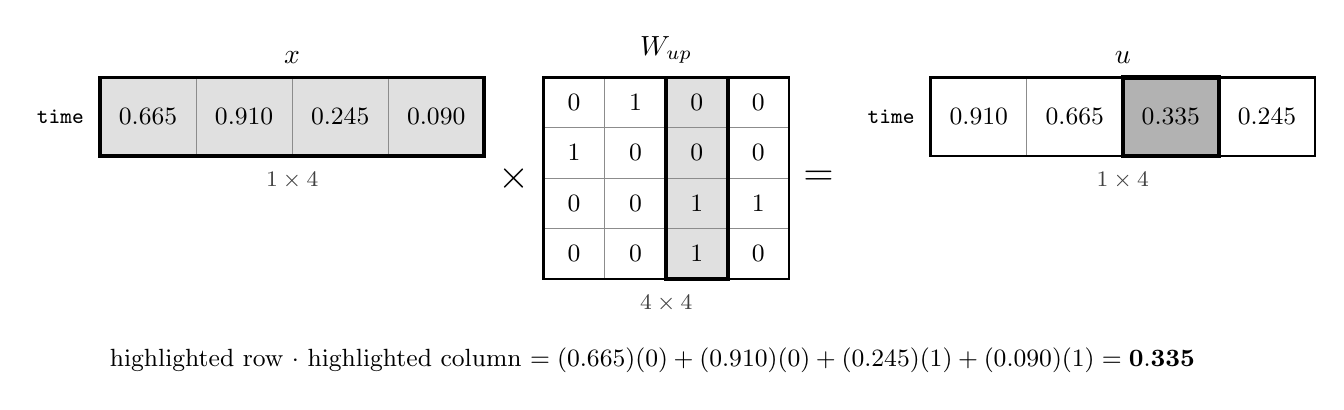
\begin{tikzpicture}
\draw[black!45, fill=black!12] (0.000,0.000) rectangle (1.220,-1.000);
\node[font=\small, text=black] at (0.610,-0.500) {$0.665$};
\draw[black!45, fill=black!12] (1.220,0.000) rectangle (2.440,-1.000);
\node[font=\small, text=black] at (1.830,-0.500) {$0.910$};
\draw[black!45, fill=black!12] (2.440,0.000) rectangle (3.660,-1.000);
\node[font=\small, text=black] at (3.050,-0.500) {$0.245$};
\draw[black!45, fill=black!12] (3.660,0.000) rectangle (4.880,-1.000);
\node[font=\small, text=black] at (4.270,-0.500) {$0.090$};
\draw[line width=1.4pt] (0.000,0.000) rectangle (4.880,-1.000);
\draw[line width=0.9pt] (0.000,0.000) rectangle (4.880,-1.000);
\node[anchor=east, font=\footnotesize\ttfamily] at (-0.080,-0.500) {time};
\node[anchor=south, font=\normalsize] at (2.440,0.050) {$\bm{x}$};
\node[anchor=north, font=\footnotesize, text=black!75] at (2.440,-1.080) {$1\times4$};
\draw[black!45, fill=white] (5.630,0.000) rectangle (6.410,-0.640);
\node[font=\small, text=black] at (6.020,-0.320) {$0$};
\draw[black!45, fill=white] (6.410,0.000) rectangle (7.190,-0.640);
\node[font=\small, text=black] at (6.800,-0.320) {$1$};
\draw[black!45, fill=black!12] (7.190,0.000) rectangle (7.970,-0.640);
\node[font=\small, text=black] at (7.580,-0.320) {$0$};
\draw[black!45, fill=white] (7.970,0.000) rectangle (8.750,-0.640);
\node[font=\small, text=black] at (8.360,-0.320) {$0$};
\draw[black!45, fill=white] (5.630,-0.640) rectangle (6.410,-1.279);
\node[font=\small, text=black] at (6.020,-0.959) {$1$};
\draw[black!45, fill=white] (6.410,-0.640) rectangle (7.190,-1.279);
\node[font=\small, text=black] at (6.800,-0.959) {$0$};
\draw[black!45, fill=black!12] (7.190,-0.640) rectangle (7.970,-1.279);
\node[font=\small, text=black] at (7.580,-0.959) {$0$};
\draw[black!45, fill=white] (7.970,-0.640) rectangle (8.750,-1.279);
\node[font=\small, text=black] at (8.360,-0.959) {$0$};
\draw[black!45, fill=white] (5.630,-1.279) rectangle (6.410,-1.919);
\node[font=\small, text=black] at (6.020,-1.599) {$0$};
\draw[black!45, fill=white] (6.410,-1.279) rectangle (7.190,-1.919);
\node[font=\small, text=black] at (6.800,-1.599) {$0$};
\draw[black!45, fill=black!12] (7.190,-1.279) rectangle (7.970,-1.919);
\node[font=\small, text=black] at (7.580,-1.599) {$1$};
\draw[black!45, fill=white] (7.970,-1.279) rectangle (8.750,-1.919);
\node[font=\small, text=black] at (8.360,-1.599) {$1$};
\draw[black!45, fill=white] (5.630,-1.919) rectangle (6.410,-2.558);
\node[font=\small, text=black] at (6.020,-2.239) {$0$};
\draw[black!45, fill=white] (6.410,-1.919) rectangle (7.190,-2.558);
\node[font=\small, text=black] at (6.800,-2.239) {$0$};
\draw[black!45, fill=black!12] (7.190,-1.919) rectangle (7.970,-2.558);
\node[font=\small, text=black] at (7.580,-2.239) {$1$};
\draw[black!45, fill=white] (7.970,-1.919) rectangle (8.750,-2.558);
\node[font=\small, text=black] at (8.360,-2.239) {$0$};
\draw[line width=1.4pt] (7.190,0.000) rectangle (7.970,-2.558);
\draw[line width=0.9pt] (5.630,0.000) rectangle (8.750,-2.558);
\node[anchor=south, font=\normalsize] at (7.190,0.050) {$W_{\text{up}}$};
\node[anchor=north, font=\footnotesize, text=black!75] at (7.190,-2.638) {$4\times4$};
\draw[black!45, fill=white] (10.550,0.000) rectangle (11.770,-1.000);
\node[font=\small, text=black] at (11.160,-0.500) {$0.910$};
\draw[black!45, fill=white] (11.770,0.000) rectangle (12.990,-1.000);
\node[font=\small, text=black] at (12.380,-0.500) {$0.665$};
\draw[black!45, fill=black!30] (12.990,0.000) rectangle (14.210,-1.000);
\node[font=\small, text=black] at (13.600,-0.500) {$0.335$};
\draw[black!45, fill=white] (14.210,0.000) rectangle (15.430,-1.000);
\node[font=\small, text=black] at (14.820,-0.500) {$0.245$};
\draw[line width=1.6pt] (12.990,0.000) rectangle (14.210,-1.000);
\draw[line width=0.9pt] (10.550,0.000) rectangle (15.430,-1.000);
\node[anchor=east, font=\footnotesize\ttfamily] at (10.470,-0.500) {time};
\node[anchor=south, font=\normalsize] at (12.990,0.050) {$\bm{u}$};
\node[anchor=north, font=\footnotesize, text=black!75] at (12.990,-1.080) {$1\times4$};
\node[font=\Large] at (5.255,-1.279) {$\times$};
\node[font=\Large] at (9.125,-1.279) {$=$};
\node[anchor=north west, font=\small] at (0,-3.308) {highlighted row $\cdot$ highlighted column $= (0.665)(0) + (0.910)(0) + (0.245)(1) + (0.090)(1) = \mathbf{0.335}$};
\end{tikzpicture}}
\\[10pt]
\nTenFit{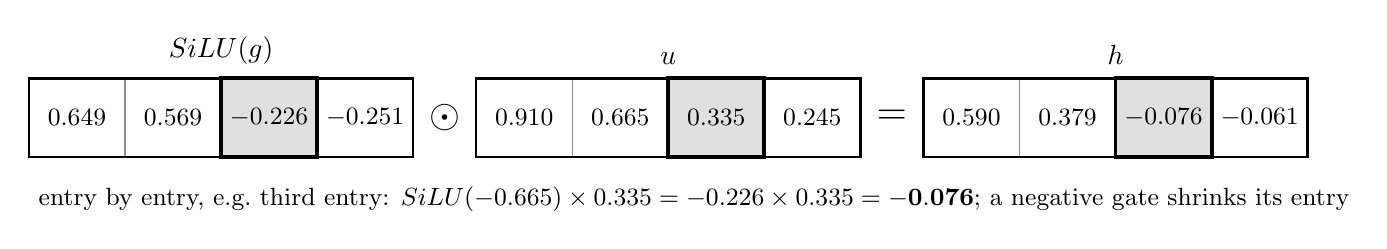
\begin{tikzpicture}
\draw[black!45, fill=white] (0.000,0.000) rectangle (1.220,-1.000);
\node[font=\small, text=black] at (0.610,-0.500) {$0.649$};
\draw[black!45, fill=white] (1.220,0.000) rectangle (2.440,-1.000);
\node[font=\small, text=black] at (1.830,-0.500) {$0.569$};
\draw[black!45, fill=black!12] (2.440,0.000) rectangle (3.660,-1.000);
\node[font=\small, text=black] at (3.050,-0.500) {$-0.226$};
\draw[black!45, fill=white] (3.660,0.000) rectangle (4.880,-1.000);
\node[font=\small, text=black] at (4.270,-0.500) {$-0.251$};
\draw[line width=1.4pt] (2.440,0.000) rectangle (3.660,-1.000);
\draw[line width=0.9pt] (0.000,0.000) rectangle (4.880,-1.000);
\node[anchor=south, font=\normalsize] at (2.440,0.050) {$\operatorname{SiLU}(\bm{g})$};
\node[font=\Large] at (5.280,-0.500) {$\odot$};
\draw[black!45, fill=white] (5.680,0.000) rectangle (6.900,-1.000);
\node[font=\small, text=black] at (6.290,-0.500) {$0.910$};
\draw[black!45, fill=white] (6.900,0.000) rectangle (8.120,-1.000);
\node[font=\small, text=black] at (7.510,-0.500) {$0.665$};
\draw[black!45, fill=black!12] (8.120,0.000) rectangle (9.340,-1.000);
\node[font=\small, text=black] at (8.730,-0.500) {$0.335$};
\draw[black!45, fill=white] (9.340,0.000) rectangle (10.560,-1.000);
\node[font=\small, text=black] at (9.950,-0.500) {$0.245$};
\draw[line width=1.4pt] (8.120,0.000) rectangle (9.340,-1.000);
\draw[line width=0.9pt] (5.680,0.000) rectangle (10.560,-1.000);
\node[anchor=south, font=\normalsize] at (8.120,0.050) {$\bm{u}$};
\node[font=\Large] at (10.960,-0.500) {$=$};
\draw[black!45, fill=white] (11.360,0.000) rectangle (12.580,-1.000);
\node[font=\small, text=black] at (11.970,-0.500) {$0.590$};
\draw[black!45, fill=white] (12.580,0.000) rectangle (13.800,-1.000);
\node[font=\small, text=black] at (13.190,-0.500) {$0.379$};
\draw[black!45, fill=black!12] (13.800,0.000) rectangle (15.020,-1.000);
\node[font=\small, text=black] at (14.410,-0.500) {$-0.076$};
\draw[black!45, fill=white] (15.020,0.000) rectangle (16.240,-1.000);
\node[font=\small, text=black] at (15.630,-0.500) {$-0.061$};
\draw[line width=1.4pt] (13.800,0.000) rectangle (15.020,-1.000);
\draw[line width=0.9pt] (11.360,0.000) rectangle (16.240,-1.000);
\node[anchor=south, font=\normalsize] at (13.800,0.050) {$\bm{h}$};
\node[anchor=north west, font=\small] at (0,-1.25) {entry by entry, e.g.\ third entry: $\operatorname{SiLU}(-0.665) \times 0.335 = -0.226\times0.335 = \mathbf{-0.076}$; a negative gate shrinks its entry};
\end{tikzpicture}}
\\[10pt]
\nTenFit{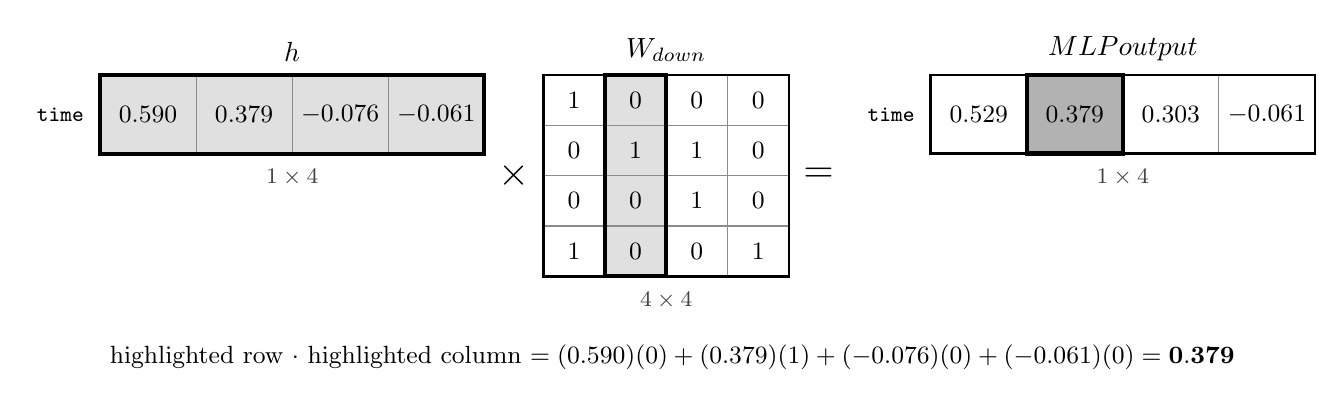
\begin{tikzpicture}
\draw[black!45, fill=black!12] (0.000,0.000) rectangle (1.220,-1.000);
\node[font=\small, text=black] at (0.610,-0.500) {$0.590$};
\draw[black!45, fill=black!12] (1.220,0.000) rectangle (2.440,-1.000);
\node[font=\small, text=black] at (1.830,-0.500) {$0.379$};
\draw[black!45, fill=black!12] (2.440,0.000) rectangle (3.660,-1.000);
\node[font=\small, text=black] at (3.050,-0.500) {$-0.076$};
\draw[black!45, fill=black!12] (3.660,0.000) rectangle (4.880,-1.000);
\node[font=\small, text=black] at (4.270,-0.500) {$-0.061$};
\draw[line width=1.4pt] (0.000,0.000) rectangle (4.880,-1.000);
\draw[line width=0.9pt] (0.000,0.000) rectangle (4.880,-1.000);
\node[anchor=east, font=\footnotesize\ttfamily] at (-0.080,-0.500) {time};
\node[anchor=south, font=\normalsize] at (2.440,0.050) {$\bm{h}$};
\node[anchor=north, font=\footnotesize, text=black!75] at (2.440,-1.080) {$1\times4$};
\draw[black!45, fill=white] (5.630,0.000) rectangle (6.410,-0.640);
\node[font=\small, text=black] at (6.020,-0.320) {$1$};
\draw[black!45, fill=black!12] (6.410,0.000) rectangle (7.190,-0.640);
\node[font=\small, text=black] at (6.800,-0.320) {$0$};
\draw[black!45, fill=white] (7.190,0.000) rectangle (7.970,-0.640);
\node[font=\small, text=black] at (7.580,-0.320) {$0$};
\draw[black!45, fill=white] (7.970,0.000) rectangle (8.750,-0.640);
\node[font=\small, text=black] at (8.360,-0.320) {$0$};
\draw[black!45, fill=white] (5.630,-0.640) rectangle (6.410,-1.279);
\node[font=\small, text=black] at (6.020,-0.959) {$0$};
\draw[black!45, fill=black!12] (6.410,-0.640) rectangle (7.190,-1.279);
\node[font=\small, text=black] at (6.800,-0.959) {$1$};
\draw[black!45, fill=white] (7.190,-0.640) rectangle (7.970,-1.279);
\node[font=\small, text=black] at (7.580,-0.959) {$1$};
\draw[black!45, fill=white] (7.970,-0.640) rectangle (8.750,-1.279);
\node[font=\small, text=black] at (8.360,-0.959) {$0$};
\draw[black!45, fill=white] (5.630,-1.279) rectangle (6.410,-1.919);
\node[font=\small, text=black] at (6.020,-1.599) {$0$};
\draw[black!45, fill=black!12] (6.410,-1.279) rectangle (7.190,-1.919);
\node[font=\small, text=black] at (6.800,-1.599) {$0$};
\draw[black!45, fill=white] (7.190,-1.279) rectangle (7.970,-1.919);
\node[font=\small, text=black] at (7.580,-1.599) {$1$};
\draw[black!45, fill=white] (7.970,-1.279) rectangle (8.750,-1.919);
\node[font=\small, text=black] at (8.360,-1.599) {$0$};
\draw[black!45, fill=white] (5.630,-1.919) rectangle (6.410,-2.558);
\node[font=\small, text=black] at (6.020,-2.239) {$1$};
\draw[black!45, fill=black!12] (6.410,-1.919) rectangle (7.190,-2.558);
\node[font=\small, text=black] at (6.800,-2.239) {$0$};
\draw[black!45, fill=white] (7.190,-1.919) rectangle (7.970,-2.558);
\node[font=\small, text=black] at (7.580,-2.239) {$0$};
\draw[black!45, fill=white] (7.970,-1.919) rectangle (8.750,-2.558);
\node[font=\small, text=black] at (8.360,-2.239) {$1$};
\draw[line width=1.4pt] (6.410,0.000) rectangle (7.190,-2.558);
\draw[line width=0.9pt] (5.630,0.000) rectangle (8.750,-2.558);
\node[anchor=south, font=\normalsize] at (7.190,0.050) {$W_{\text{down}}$};
\node[anchor=north, font=\footnotesize, text=black!75] at (7.190,-2.638) {$4\times4$};
\draw[black!45, fill=white] (10.550,0.000) rectangle (11.770,-1.000);
\node[font=\small, text=black] at (11.160,-0.500) {$0.529$};
\draw[black!45, fill=black!30] (11.770,0.000) rectangle (12.990,-1.000);
\node[font=\small, text=black] at (12.380,-0.500) {$0.379$};
\draw[black!45, fill=white] (12.990,0.000) rectangle (14.210,-1.000);
\node[font=\small, text=black] at (13.600,-0.500) {$0.303$};
\draw[black!45, fill=white] (14.210,0.000) rectangle (15.430,-1.000);
\node[font=\small, text=black] at (14.820,-0.500) {$-0.061$};
\draw[line width=1.6pt] (11.770,0.000) rectangle (12.990,-1.000);
\draw[line width=0.9pt] (10.550,0.000) rectangle (15.430,-1.000);
\node[anchor=east, font=\footnotesize\ttfamily] at (10.470,-0.500) {time};
\node[anchor=south, font=\normalsize] at (12.990,0.050) {$\text{MLP output}$};
\node[anchor=north, font=\footnotesize, text=black!75] at (12.990,-1.080) {$1\times4$};
\node[font=\Large] at (5.255,-1.279) {$\times$};
\node[font=\Large] at (9.125,-1.279) {$=$};
\node[anchor=north west, font=\small] at (0,-3.308) {highlighted row $\cdot$ highlighted column $= (0.590)(0) + (0.379)(1) + (-0.076)(0) + (-0.061)(0) = \mathbf{0.379}$};
\end{tikzpicture}}
